\section{Background}
A major concern with real-time image processing, especially in first responder situations, is speed. Because FPGAs have the ability to process data in parallel, they are ideal for this type of application. Using an FPGA for this system will enable all data inputs to be processed at the same time, thereby dramatically increasing throughput speed. Since everything is running in parallel, more data inputs can be added to the system to increase functionality without introducing any latency into the system, as long as enough memory and hardware are available.
\par
SLAM is a widely expanding field with much potential for improvement. One application of such a system is a proof of concept of camera-based SLAM systems, presented by Andrew Davison of Oxford University in a research paper entitled ''Real-Time SLAM with a Single Camera'' \cite{davison}. This system is handheld and relies on a computer using a 2.2 GHz Pentium processor connected to a single camera and laser rangefinder. The system requires prior knowledge of the area being analyzed before it can successfully localize and map. It implements edge detection, but is limited to the narrow field of vision of the rangefinder, so it is only able to map an object directly in front of it. This system carries a latency of around 33 milliseconds. An output frame of the device is shown in Figure \ref{rtSLAM}.

\begin{figure}[H]
	\centerline{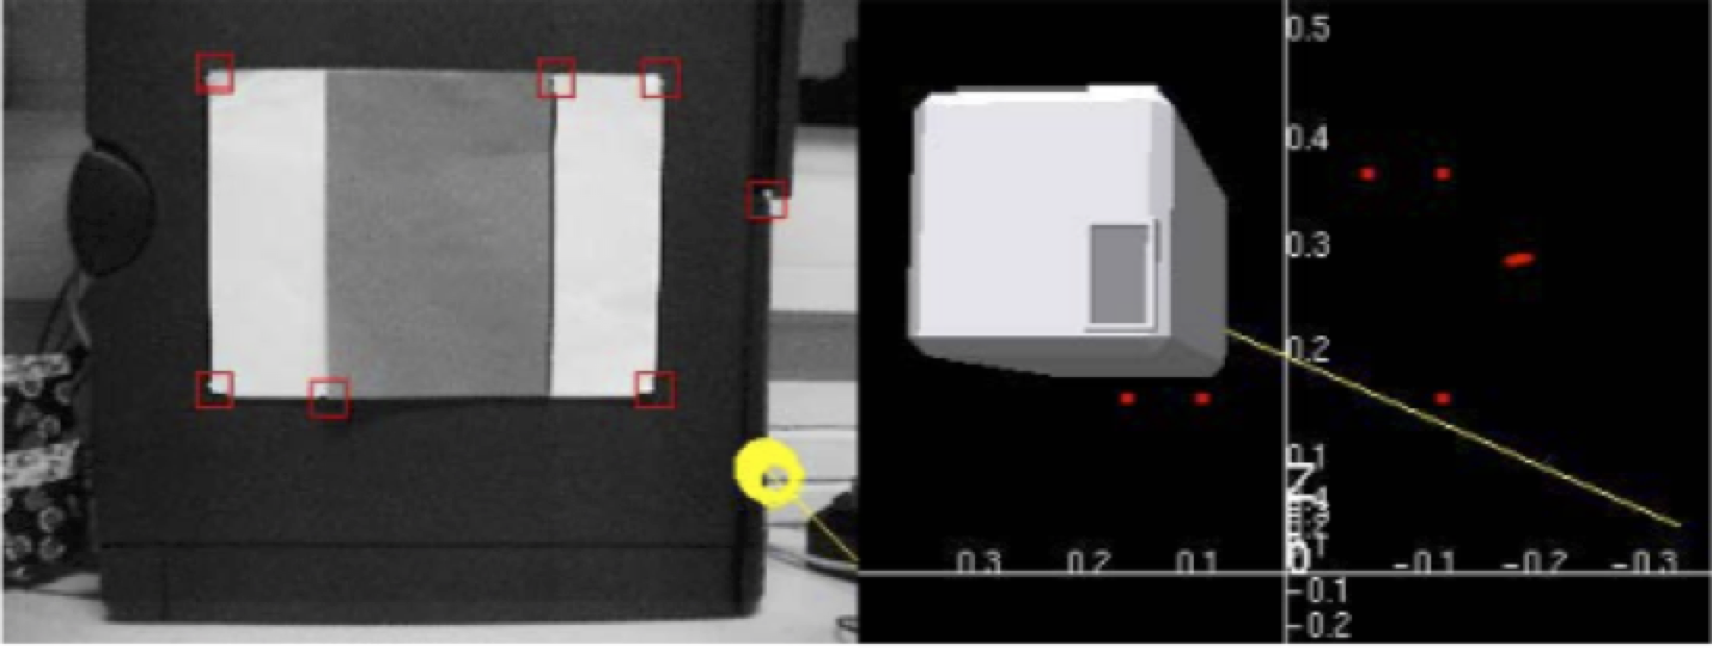
\includegraphics[width=0.8\textwidth]{real_time_SLAM.png}}
	\caption{Real-Time SLAM with a Single Camera \cite{davison}}
	\label{rtSLAM}
\end{figure}

The frame on the left in Figure \ref{rtSLAM} is the video feed with 6 points of a paper target input as prior knowledge, along with successfully marked identifying features (marked as red squares), and another identifying feature that is not marked for measurement (marked by a yellow circle). The frame on the right is a localization graph displaying the positions of all red squares.
\par
A more commercial device similar to our concept is Serveball's Squito\textsuperscript{TM} \cite{serveball}. Squito is a wireless, throwable, 360$^{\circ}$ panoramic camera that implements target detection to stabilize the video feed from its many cameras. It is shown in Figure \ref{squito} below.

\begin{figure}[H]
	\centerline{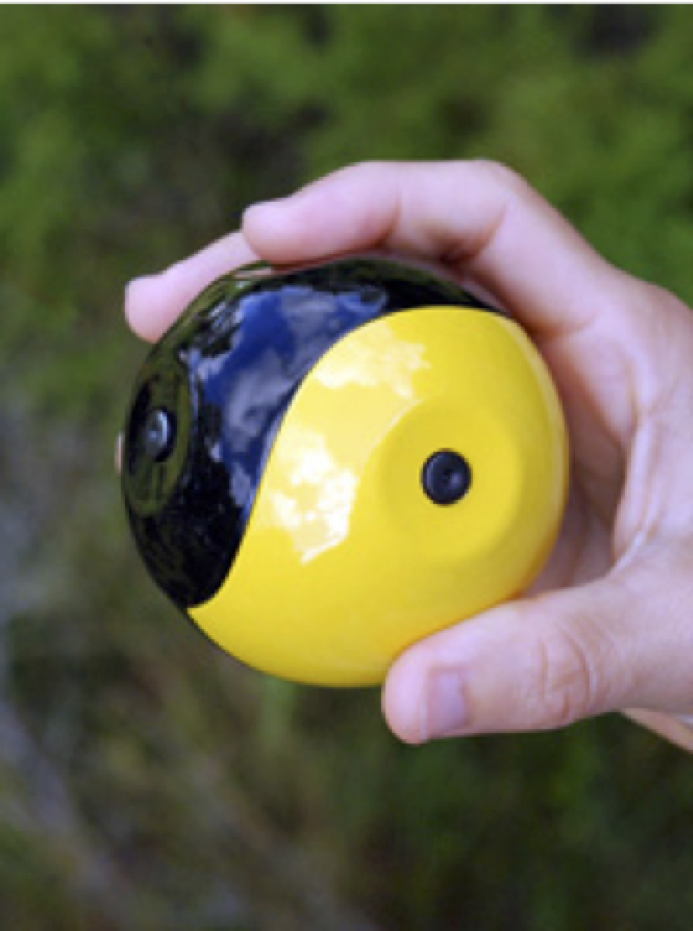
\includegraphics[width=0.3\textwidth]{serveball_squito.png}}
	\caption{Serveball's Squito \cite{serveball}}
	\label{squito}
\end{figure}

Squito utilizes a microprocessor receiving input from cameras, as well as orientation and position sensors, in order to transmit a real-time stabilized video of its adventure. The device is still in the prototype stage and is receiving interest from first responders. The image in Figure \ref{squito_io} shows the input from the Squito's four cameras on the left, and the corresponding stitched output on the right.

\begin{figure}[H]
	\centerline{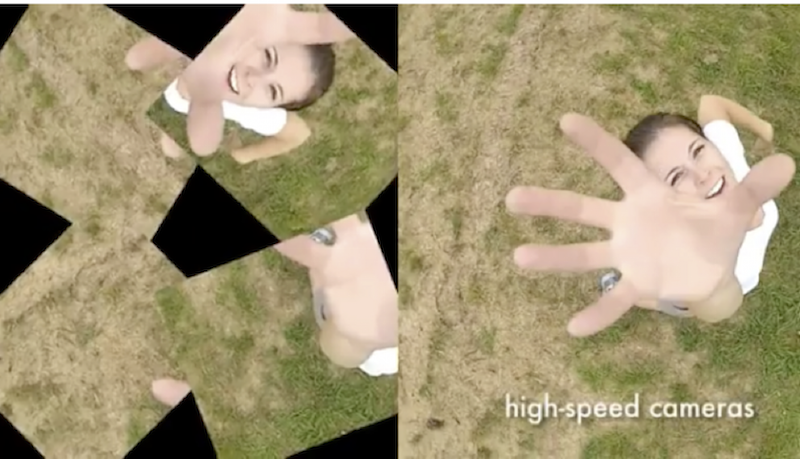
\includegraphics[width=0.6\textwidth]{serveball_io.png}}
	\caption{Serveball's Squito Input and Output \cite{serveball}}
	\label{squito_io}
\end{figure}

By using multiple camera sensors in a sensor suite, it is also possible to determine depth information from corresponding images of an area. This technique is known as stereo imaging, and the process of gathering depth information from a pair of stereo images is known as disparity mapping. University of Bologna researchers Stefano Mattoccia and Matteo Poggi have worked to implement a real-time disparity mapping algorithm on an FPGA, and an example of a stereo image disparity is shown in Figure \ref{disparity_example} below \cite{mattoccia}. Using their stereo vision algorithm, the researchers are able to generate real-time image data showing the relative locations of objects within an image frame using color gradients. Based on this depth information, it is also possible to detect objects located within the field of view of the stereo imaging system, as shown in Figure \ref{disparity_example}. An implementation similar to this is extremely useful in a SLAM-like system, as it would allow for the localization of objects and creation of 2D "floorplans" of an area in real-time using only two camera sensors.

\begin{figure}[H]
	\centerline{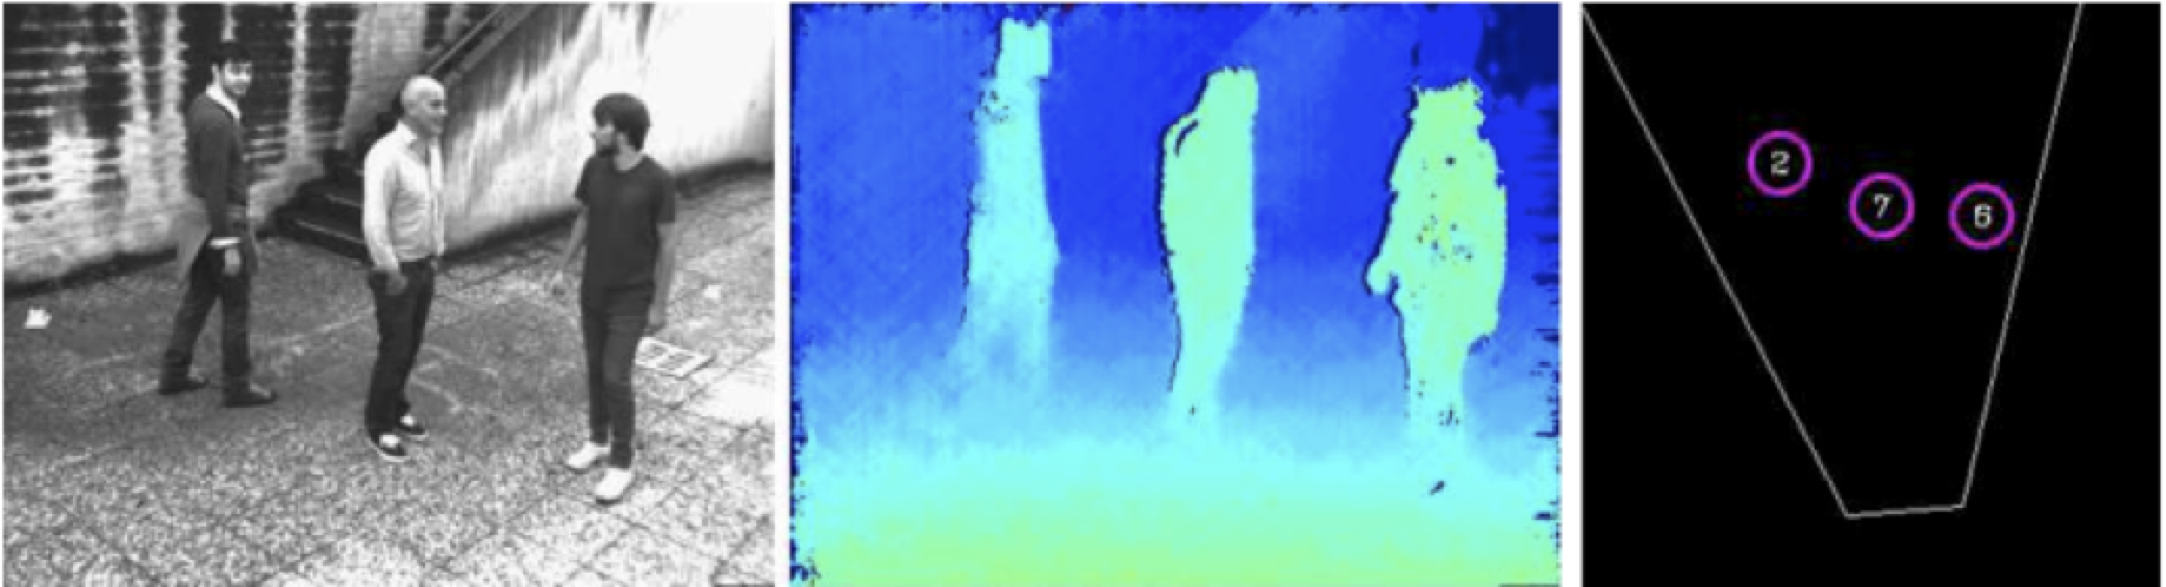
\includegraphics[width=0.9\textwidth]{disparity_example.png}}
	\caption{From Left to Right: Original Image, Disparity Map, Object Detection Results \cite{mattoccia}}
	\label{disparity_example}
\end{figure}

Many security systems implement human detection and human body tracking in order to increase their effectiveness. These devices process real-time images in order to identify human characteristics, and are limited to the field of vision of a stationary or rotating camera. An example of this type of system is explored by the Mitsubishi corporation in a research paper entitled "Human Body Tracking by Adaptive Background Models and Mean-Shift Analysis" \cite{porikli}. The paper explores a stationary image processing system implemented on a PC platform with a 1.8GHz processor that yields a maximum processing time of 100 milliseconds. An output frame of the system is shown in Figure \ref{human_tracking} below.

\begin{figure}[H]
	\centerline{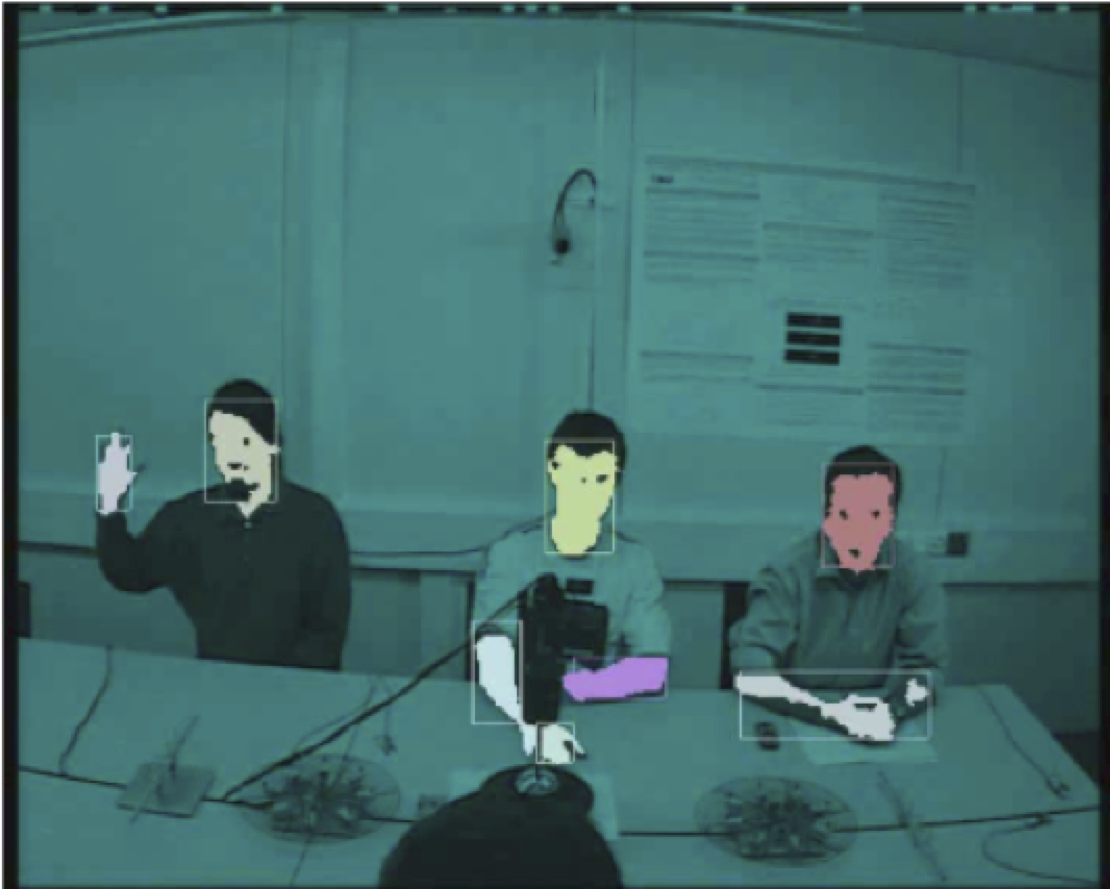
\includegraphics[width=0.5\textwidth]{human_tracking.png}}
	\caption{\small{Human Body Tracking by Adaptive Background Models and Mean-Shift Analysis \cite{porikli}}}
	\label{human_tracking}
\end{figure}

The proposed device would ideally combine the ideas of the four systems examined. However, due to project time constraints we focused on SLAM-based area mapping, and have recommended the future addition of human detection algorithms. The proposed device would be capable of generating real-time 2D maps of the area it is traversing, as well as a 3D depth map of the device’s current field of view.
\par
In order to successfully implement this system, we proposed the creation of a device that would rely on two stereo cameras, a laser rangefinder, and an inertial measurement unit (IMU) as its sensor suite, as shown in Appendix Item \ref{componentSelection}. Little to no comparable existing commercial products were capable of processing their gathered data locally and in real-time. Stereo cameras would allow our device to calculate disparity, just as human eyes do. Although disparity is useful for localization, it is not enough for accurate mapping because it only accurately provides the relative distance between objects. The inclusion of a rangefinder would allow for precise base distance readings, and an IMU would be used to localize all gathered data. All of this data was then combined with the disparity maps and image data in order to create flawless localization and mapping. All time-dependent processing required for the device would be mainly done in parallel using hardware on an FPGA, in order to reduce system latency. An overall functional block diagram of our intended implementation is shown in Figure \ref{orig_bd} below.

\begin{figure}[H]
	\centerline{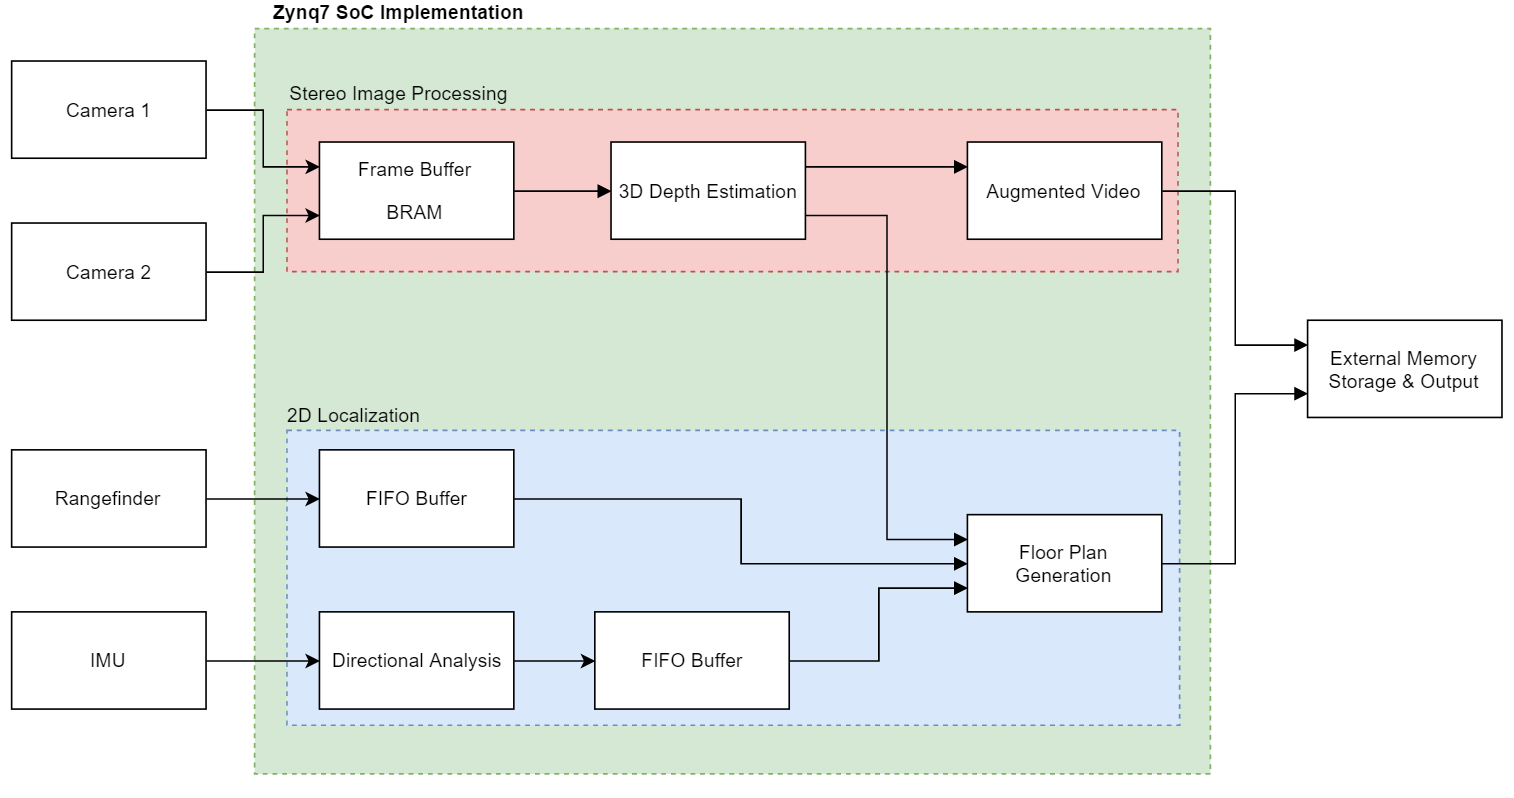
\includegraphics[width=1.2\textwidth]{block_diagram.png}}
	\caption{Functional Block Diagram}
	\label{orig_bd}
\end{figure}

Most applicable previous camera-based systems have also focused on mapping from a stationary point, or edge detection from a mobile platform. Our project aimed to combine these concepts, by creating a mobile mapping device that would be especially of use in many first responder situations.
\par
As our research has progressed over time, the project objectives have continually evolved. We originally envisioned the creation of a device that used laser rangefinders to create 3D maps of its surroundings, similar to that of a Carnegie Mellon University device created in order to volumetrically map abandoned mines \cite{thrun}.
\par
As our research progressed, we believed that we could use visual light and thermal imaging camera set to gather information on an area, and supplement that data with IMU and rangefinder readings in order to product detailed maps of the sensor suite's surroundings. Eventually we came upon the concept of disparity mapping and generating depth information from image data, and decided that we would again like to shift the overall setup of our device to rely mainly on stereo image data. Due to our overall budget, time constraints, and the resources that have been made available to us, in the coming terms we planned to use an electronic scanning laser rangefinder, IMU, and stereo camera pair to generate real-time SLAM video and floorplan information. Although we were also originally planning on including a thermal camera in our sensor suite as well, we decided to eliminate the module in favor of higher quality cameras due to its prohibitive cost, low resolution, slow sampling rate, and small field of view. We also originally proposed the inclusion of human object detection in our project, but modified our proposal and included it as a future suggestion due to project time constraints.




